% The packed two-pass traversal of the element operators on the CPU: elements in packs with local
% 16-bit node numbers, each node owned by one pack; pass 1 runs a pack per thread task into
% thread-local scratch, writes its owned nodes and parks its ghost contributions; pass 2 adds the
% parked contributions to their nodes in a fixed order.  No atomics; the result is deterministic.
\documentclass[border=2pt]{standalone}
% Shared preamble of the format diagrams: colours of the paper's figures (paper_figures.py) and
% the drawing styles.  Each diagram is a standalone document built to a PDF of the text width.
\usepackage{amsmath,amssymb}
\usepackage{tikz}
\usetikzlibrary{arrows.meta,calc,decorations.pathreplacing,patterns,positioning}

\definecolor{cindex}{HTML}{BDBDBD}  % column indices, offsets, row pointers
\definecolor{cvalue}{HTML}{6E6E6E}  % floating-point values (BSR)
\definecolor{cpoint}{HTML}{1B9E77}  % quadrature-point store
\definecolor{celem}{HTML}{1F78B4}   % element matrix
\definecolor{cqbsr}{HTML}{A6761D}   % quantized BSR
\definecolor{cscale}{HTML}{E6AB02}  % scales
\definecolor{cmean}{HTML}{7570B3}   % f32 element mean

\tikzset{
  >={Stealth[length=4pt]},
  grid/.style={draw=black!45, line width=0.25pt},
  frame/.style={draw=black!70, line width=0.5pt},
  title/.style={font=\small\bfseries, anchor=west, inner sep=0pt},
  lab/.style={font=\footnotesize, inner sep=1pt},
  note/.style={font=\scriptsize, text=black!75, inner sep=1pt, execute at begin node={\hyphenpenalty=10000\exhyphenpenalty=10000}},
  num/.style={font=\tiny, inner sep=0pt},
  brace/.style={decorate, decoration={brace, amplitude=3pt, raise=1pt}, line width=0.4pt},
  arr/.style={->, line width=0.5pt, black!70},
  pad/.style={pattern=north east lines, pattern color=black!30},
}

% \cell{x}{y}{w}{h}{fill}: a filled rectangle with a thin outline, lower-left corner at (x,y).
\newcommand{\cell}[5]{\filldraw[fill=#5, grid] (#1,#2) rectangle ++(#3,#4);}
% \blk{x}{y}{s}{fill}: a 3x3 block of side s with its 3x3 entry grid.
\newcommand{\blk}[4]{%
  \filldraw[fill=#4, grid] (#1,#2) rectangle ++(#3,#3);
  \draw[draw=white, line width=0.25pt] (#1,#2) ++(#3/3,0) -- ++(0,#3) ++(#3/3,0) -- ++(0,-#3);
  \draw[draw=white, line width=0.25pt] (#1,#2) ++(0,#3/3) -- ++(#3,0) ++(0,#3/3) -- ++(-#3,0);
  \draw[grid] (#1,#2) rectangle ++(#3,#3);}
% \vthree{x}{y}{fill}: a 3-vector (one node's components) as three small cells, left end at (x,y).
\newcommand{\vthree}[3]{\foreach \k in {0,1,2} \filldraw[fill=#3, grid] (#1+\k*0.14,#2) rectangle ++(0.14,0.14);}
% \op{x}{y}{symbol}: an operation in a small circle.
\newcommand{\op}[3]{\node[circle, draw=black!70, line width=0.4pt, inner sep=0.5pt, minimum size=9pt, font=\tiny] at (#1,#2) {#3};}

\begin{document}
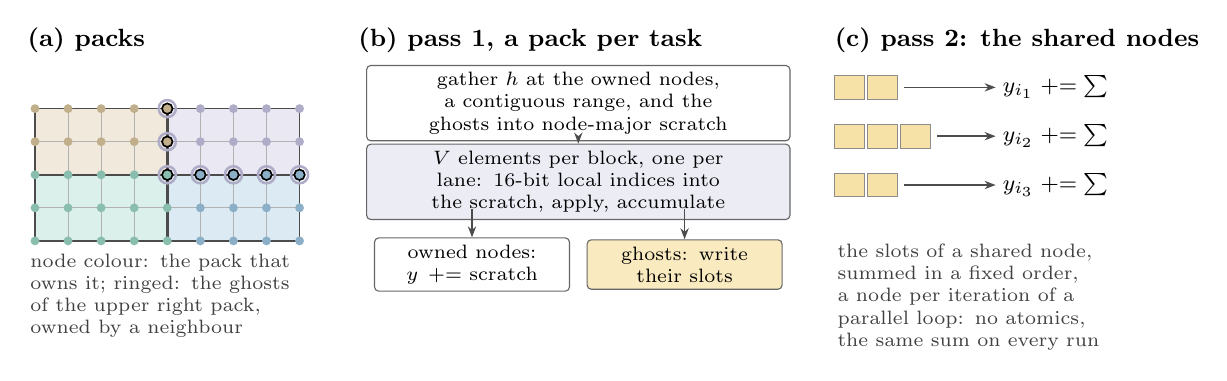
\begin{tikzpicture}
  \colorlet{pk0}{cpoint!45}\colorlet{pk1}{celem!45}\colorlet{pk2}{cqbsr!45}\colorlet{pk3}{cmean!45}
  \tikzset{
    stage/.style={draw=black!60, line width=0.4pt, rounded corners=1.5pt, font=\scriptsize, align=center,
                  inner sep=2.5pt, minimum height=0.55cm},
  }
  % ---------------------------------------------------------------- (a) packs
  \node[title] at (0, 3.3) {(a) packs};
  \def\q{0.42}
  \begin{scope}[shift={(0.1,0.75)}]
    \foreach \ci in {0,...,7} \foreach \cj in {0,...,3} {
      \pgfmathtruncatemacro{\p}{(\ci>=4) + 2*(\cj>=2)}
      \filldraw[fill=pk\p!35, draw=black!30, line width=0.25pt] (\ci*\q,\cj*\q) rectangle ++(\q,\q);
    }
    \draw[frame, line width=0.9pt] (4*\q,0) -- (4*\q,4*\q) (0,2*\q) -- (8*\q,2*\q);
    \draw[frame] (0,0) rectangle (8*\q,4*\q);
    \foreach \i in {0,...,8} \foreach \j in {0,...,4} {
      \pgfmathtruncatemacro{\o}{(\i>=5) + 2*(\j>=3)}
      \pgfmathtruncatemacro{\g}{(\i>=4 && \j>=2 && \o!=3) ? 1 : 0}
      \ifnum\g=1
        \filldraw[fill=pk\o!90!black, draw=black, line width=0.6pt] (\i*\q,\j*\q) circle (1.9pt);
        \draw[pk3!90!black, line width=0.9pt] (\i*\q,\j*\q) circle (3.1pt);
      \else
        \fill[pk\o!90!black] (\i*\q,\j*\q) circle (1.6pt);
      \fi
    }
    \node[note, anchor=north west, align=left, text width=3.6cm] at (-0.1,-0.12)
      {node colour: the pack that owns it; ringed: the ghosts of the upper right pack, owned by a neighbour};
  \end{scope}

  % ---------------------------------------------------------------- (b) pass 1
  \begin{scope}[shift={(4.2,0)}]
    \node[title] at (0, 3.3) {(b) pass 1, a pack per task};
    \node[stage, fill=white, text width=5.2cm] (g) at (2.8,2.5)
      {gather $h$ at the owned nodes, a contiguous range, and the ghosts into node-major scratch};
    \node[stage, fill=pk3!30, text width=5.2cm] (e) at (2.8,1.5)
      {$V$ elements per block, one per lane: $16$-bit local indices into the scratch, apply, accumulate};
    \node[stage, fill=white, text width=2.3cm] (o) at (1.45,0.45) {owned nodes:\\$y \mathrel{+}=$ scratch};
    \node[stage, fill=cscale!25, text width=2.3cm] (s) at (4.15,0.45) {ghosts: write\\their slots};
    \draw[arr] (g) -- (e); \draw[arr] (1.45,1.15) -- (o); \draw[arr] (4.15,1.15) -- (s);
  \end{scope}

  % ---------------------------------------------------------------- (c) pass 2
  \begin{scope}[shift={(10.25,0)}]
    \node[title] at (0, 3.3) {(c) pass 2: the shared nodes};
    \foreach \r/\n [count=\i from 0] in {2/{i_1}, 3/{i_2}, 2/{i_3}} {
      \pgfmathsetmacro{\y}{2.55-\i*0.62}
      \foreach \k in {1,...,\r} {\pgfmathsetmacro{\x}{(\k-1)*0.42}\cell{\x}{\y}{0.38}{0.3}{cscale!35}}
      \draw[arr] (\r*0.42+0.05,\y+0.15) -- (2.05,\y+0.15);
      \node[lab, anchor=west] at (2.1,\y+0.15) {$y_{\n} \mathrel{+}= \sum$};
    }
    \node[note, anchor=north west, align=left, text width=3.6cm] at (0,0.75)
      {the slots of a shared node, summed in a fixed order, a node per iteration of a parallel loop: no atomics, the same sum on every run};
  \end{scope}
\end{tikzpicture}
\end{document}
